% !TeX root = ../tfg.tex
% !TeX encoding = utf8


\chapter{Aproximación de operadores no lineales mediante redes neuronales}\label{ch:sexto-capitulo}

En las últimas décadas, la mayoría de avances en el campo del aprendizaje profundo han estado inspirados en el Teorema de Aproximación Universal~\cite{cybenko1989approximation} publicado por  George Cybenko en el año 1989. En él, se demuestra que las funciones de tipo $ \sum_{j=1}^n \alpha_{j}\sigma(w_{j}^T x + \theta_j)$, que definen una red neuronal con una única capa oculta y activación sigmoidal, son densas en el espacio de funciones continuas $C(I^n)$, con $I^n = [0,1]$. Unos años más tarde, en 1995, Tianping Chen y Robert Chen publican un artículo~\cite{chen1995universal} en el que se revisan las limitaciones de este teorema. En concreto, señalan las restricciones impuestas a las funciones de activación sigmoidales, que se presuponen continuas, y la incapacidad  de este tipo de redes neuronales para hacer frente a problemas regidos por funcionales u operadores no lineales. En esta sección entraremos en detalle en los avances propuestos en estas dos líneas. 

%El problema de aproximación de funcionales, aunque había sido abordado previamente ~\cite{Sandberg1992}, no se había hecho de forma explícita. 
\section{Notación y definiciones}
Comenzaremos aclarando algunos conceptos clave para seguir las demostraciones de esta sección: 
\begin{definicion}
Una función $\sigma:\mathds{R}\rightarrow\mathds{R}$ es sigmoidal si cumple
\begin{gather}
\sigma(x) = 
\begin{cases}
	\lim_{x\rightarrow - \infty}\sigma (x) = 0  \\
	\lim_{x\rightarrow \infty}\sigma (x) = 1.  		\end{cases}
\end{gather}
\end{definicion}
\begin{observacion}
A diferencia de otras definiciones, cuando nos refiramos a una función sigmoidal no vamos a presuponer continuidad ni monotonía.
\end{observacion}

\begin{definicion}
Una función $g:\mathds{R}\rightarrow \mathds{R}$ se llama de Tauber-Wiener (TW) si satisface que todas las combinaciones lineales 
$\sum_{i=1}^{N}c_{i}g(\lambda_{i}x+\theta_{i})$, $ \lambda_{i}$, $\theta_{i}$, $c_{i}\in\mathds{R}$, $i=1,\ldots,N$
son densas en cualquier espacio $C[a,b]$. 
\end{definicion}

\begin{definicion}
Denotaremos por $C_{p}[-1,1]^{n}$ al espacio de las funciones periódicas con respecto a cada variable $x_{1},\ldots,x_{n}$ cuyo periodo es $2$. 
\end{definicion}
\section{Características de las funciones de activación}

En esta sección trabajaremos en debilitar las condiciones bajo las cuales una función puede ser considerada función de activación, lo que nos dará más libertad a la hora de trabajar con operadores no lineales en la próxima sección. El resultado más importante es el \autoref{thm:p03}, que nos dice que pertenecer a la clase $(TW)$ es condición suficiente para que una función sea de activación.  Como las funciones $(TW)$ toman valores en $\mathds{R}$, vamos a poder trabajar con problemas simplificados.  La convergencia uniforme que nos da este teorema va a ser muy importante para los resultados de la sección siguiente. 
\begin{teorema}\label{thm:p01}
Supongamos que g es una función continua y $g\in S'(\mathds{R})$ vista como distribución. Entonces \(g\in(TW)\) si $g$ no es un polinomio. 
\end{teorema}


\begin{proof}[Demostración]
Si las combinaciones \( \sum_{i=1}^{N} c_{i}g(\lambda_{i}x+\theta_{i})\), vistas como subespacio, no son densas en \( C[a,b]\) (es decir, si su cierre forma un subespacio cerrado propio en $C[a,b]$) entonces por el \hyperref[thm:h03]{Teorema de Extensión de Hahn-Banach} existe un funcional lineal y continuo $F$ cuyo núcleo se traga al subespacio. Por otra parte, el \hyperref[thm:h04]{Teorema de Representación de Riesz} asegura que hay una medida de Borel $d\mu$ con \( \mathrm{supp}(d\mu) \subseteq [a,b] \) cumpliendo que $F(f) = \int_{\mathds{R}}fd\mu$ para toda $f\in C[a,b]$. 

Como $g(\lambda x + \theta)$ está en dicho subespacio para todo $\lambda\neq 0$ y $\theta\in\mathds{R}$, por los dos resultados anteriores, sabemos que: 

\[F(g(\lambda x + \theta)) = \int_{\mathds{R}}g(\lambda x + \theta )d\mu = 0\]

para todo \(\lambda \neq 0\) y \(\theta \in \mathds{R}\). Tomando ahora cualquier \(w \in S(\mathds{R})\), tenemos que 
\begin{equation}
\int_{\mathds{R}}w(\theta)d\theta\int_{\mathds{R}}g(\lambda x + \theta)d\mu = 0 
\end{equation}
para todo $\lambda \neq 0$ y $\theta\in\mathds{R}$.  

Fijados un  $\lambda \neq 0$ y un $\theta\in\mathds{R}$, definimos la medida $\hat{d\mu}(A)= d\mu(\frac{A-\theta}{\lambda})$ y efectuamos el cambio de variable  \(y = \lambda x + \theta\). Esto nos va a permitir ver a g como distribución: 
\begin{equation}\label{eq:id04}
\int_{\mathds{R}}g(y) \int_{\mathds{R}}w(\theta)d\mu(\frac{y-\theta}{ \lambda}) = \langle \Lambda_{g}, w(\cdot)\ast d\mu (\lambda\cdot)\rangle = 0.
\end{equation}


Por el Teorema de Inversión, tenemos: 


\begin{align}\label{eq:id05}
\langle \Lambda_{g}, w(\cdot)\ast d\mu (\lambda\cdot)\rangle 
& = \langle \Lambda_{g}, \mathcal{F}(\mathcal{F}( w(\cdot)\ast d\mu (\lambda\cdot)))\rangle
= \langle \mathcal{F}(\Lambda_{g}),\mathcal{F}( w(\cdot)\ast d\mu (\lambda\cdot))\rangle \nonumber \\ &
= \langle \mathcal{F}(\Lambda_{g}),\mathcal{F}( w(\cdot))\cdot \mathcal{F}(d\mu (\lambda\cdot))\rangle = 0.
\end{align}



 Para que~\eqref{eq:id04}  tenga sentido, tenemos que probar que \([\mathcal{F}(w)](t)\cdot[\mathcal{F}(d\mu)](\lambda t)\in \mathcal{S}(\mathds{R}^{d})\). Como \(\mathrm{supp}(d\mu)\subseteq[a,b]\), podemos escribir
 
\begin{align*}\langle\mathcal{F}(d\mu),\phi\rangle & = \langle d\mu,\mathcal{F}(\phi)\rangle 
 = \int_{\mathds{R}} d\mu(t)\mathcal{F}(\phi)(t)dt 
 = \int_{\mathds{R}} \left[ \int_{\mathds{R}}\phi(x)e^{-ixt} dx\right]d\mu(t)dt
 \\
 & =  \int_{\mathds{R}} \phi(x) \left[ \int_{\mathds{R}} e^{-ixt} d\mu(t)dt \right] dx 
 =  \int_{\mathds{R}} \phi(x) h(x)dx 
 = \langle \Lambda_{h},\phi\rangle
\end{align*}
 
donde $h(x) = \int_{\mathds{R}} e^{-ixt} d\mu (t)$.
 
 
 Además, por el \hyperref[thm:h02]{Teorema de derivación bajo el signo integral} sabemos que $h\in C^{\infty}(\mathds{R})$, lo cual nos dice que $\mathcal{F}(d\mu)$ es, vista como una función, de clase $C^{\infty}(\mathds{R})$. 
 
Veamos ahora que para cada \(k=1,2,\ldots\), existe una constante \(c_{k}\) tal que:
\[\vert \frac{\partial^{k}}{\partial t^{k}} \mathcal{F}(d\mu)(t)\vert \leq c_{k}.\]


Efectivamente, tenemos que 
\begin{gather} \vert h(x)\vert = \vert \int_{\mathds{R}} e^{-ixt} d\mu (t)\vert \leq  \int_{\mathds{R}} \vert e^{-ixt} \vert \vert d\mu (t)\vert \leq  \int_{\mathds{R}}  \vert d\mu (t)\vert \leq 1, \qquad \forall x\in \mathds{R}.
\end{gather}


De forma análoga, podemos ver que 

\begin{align*}
\langle \frac{\partial^{k}}{\partial t^{k}} \mathcal{F}(d\mu),\phi\rangle &=
\langle \mathcal{F}(t^{k}d\mu),\phi\rangle = \langle t^{k}d\mu, \mathcal{F}(\phi)\rangle  = \int_{\mathds{R}} \mathcal{F} (\phi )(t)t^{k}d\mu (t)dt \\ &= 
\int_{\mathds{R}} \left[ \int_{\mathds{R}}\phi (x)e^{-ixt}t^{k}d\mu (t)dx\right]dt = \int_{\mathds{R}} \phi (x) \left[ \int_{\mathds{R}}e^{-ixt}t^{k}d\mu (t)dt\right]dx 
\\
&=  \langle \Lambda_{h_{k}},\phi \rangle
\end{align*}

donde estamos considerando  $ \Lambda_{h_{k}} = \mathcal{F}(t^{k}d\mu) $, lo cual nos permite ver a  $h_{k}$ como función. 

Desde aquí, teniendo en cuenta que $\mathrm{supp}(d\mu)\subset [a,b] $, es fácil ver que 

$$ \vert h_{k}(x)\vert \leq \int_{\mathds{R}} \vert t^{k} \vert d\mu (t)= c_{k}$$

para alguna constante $c_{k}\in \mathds{R}$.  


Como consecuencia, por ser $\mathcal{F}(w)$ de crecimiento lento y tener $\mathcal{F}(d\mu)$ todas sus derivadas acotadas,  \(\mathcal{F}(w)\cdot \mathcal{F}(d\mu)\in \mathcal{S}(\mathds{R})\). 
Por el \hyperref[thm:h04]{Teorema de Representación de Riesz} sabíamos que \(d\mu \not\equiv 0 \) y, además, hemos visto que \(\mathcal{F}(d\mu)\in C^{\infty}(\mathds{R})\). Por tanto, podemos afirmar que existe algún \(t_{0} \neq 0 \) con un entorno \((t_{0}-\delta,t_{0}+\delta)\) tal que \(\mathcal{F}(d\mu)(t) \neq 0\) para todo \(t\in (t_{0}-\delta,t_{0}+\delta)\). Si tomamos \(\lambda = \frac{t_{0}}{t_{1}}\), con \(t_{1} \neq 0\), entonces $\mathcal{F}(d\mu)(\lambda t) \neq 0
$, $ \forall t \in (t_{1}-\frac{\delta}{\lambda},t_{1}+\frac{\delta }{\lambda})$. Tomando un \(\mathcal{F}(w)\in C^{\infty}_{c}(t_{0}-\frac{\delta } {2\lambda},t_{0}+\frac{\delta } {2\lambda})\) cualquiera, entonces \(\frac{\mathcal{F}(w)}{\mathcal{F}(d\mu)(\lambda t)} \in\mathcal{S}(\mathds{R})\) y, por ~\eqref{eq:id05}:
\[\mathcal{F}(g)(\mathcal{F}(w)(\cdot)) = \mathcal{F}(g)\left(\frac{\mathcal{F}(w)(\cdot)} { \mathcal{F}(d\mu)(\lambda\cdot)}\mathcal{F}(d\mu)(\lambda\cdot)\right) = 0.\]

Acabamos de ver que para cualquier punto \(t^{*}\in\mathds{R}\) fijo, existe un entorno \([t^{*}-\eta,t^{*}+\eta]\) tal que \(\mathcal{F}(g)(\mathcal{F}(w)(\cdot))=0\) se cumple para todo \(\mathcal{F}(w)\) con soporte compacto en \([t^{*}-\eta,t^{*}+\eta]\), esto es, \(\mathrm{supp}(\mathcal{F}(g) )\subseteq \{0\}\). Por el \autoref{thm:d02}, \(\mathcal{F}(g)\) es una combinación de deltas de Dirac y sus derivadas. Lo que equivale, como vimos en el \autoref{lm:d02}, a que $g$ sea un polinomio. Con esto, el \autoref{thm:p01} queda probado. 
\end{proof}



\begin{teorema}\label{thm:p03}
Supongamos que K es un conjunto compacto en $\mathds{R}^{n}$,  $U$ es un conjunto compacto en \(C(K)\) y  \(g\in(TW)\). Entonces, para cada $\varepsilon >0$, existe un entero positivo \(N\), números reales $\theta_{i}$, vectores $w_{i}\in\mathds{R}^{n}$, $i=1,\ldots,N$, con independencia de  \(f\in U\) y constantes $c_{i}(f)$,  $i=1,\ldots,N$ dependientes de f tal que 
\[\vert f(x) - \sum_{i=1}^{N}c_{i}(f)g( w_{i} x + \theta_{i}) \vert < \varepsilon\]

se cumple para todo \(x\in K\) y para toda \(f\in U\). 
\end{teorema}


Antes de demostrar el \autoref{thm:p03}, veamos un resultado previo que nos va a ser necesario: 


\begin{lema}\label{lm:p03}
Supongamos que K es un conjunto compacto en \(I^{n} = [0,1]^{n}\) y $V$ es un conjunto compacto en $C(K)$. Entonces $V$ puede extenderse a un conjunto compacto en \(C_{p}[-1,1]^{n}\).
\end{lema}
\begin{proof}[Demostración]
Para toda $f\in V$ sabemos, por el \autoref{lm:p01}, que existe una extensión continua $E(f)\in C([0,1]^{n})$ tal que $sup_{x\in [0,1]^{n}}\{\vert E(f)(x)\vert\} \leq sup_{x\in K}\{ \vert f(x)\vert\}$. Por el \hyperref[thm:h05]{Teorema de Ascoli-Azela}, sabemos también que existe una constante $M$ tal que $\|f(x)\|_{C(K)} \leq M$, por lo que $sup_{x\in [0,1]^{n}}\{\vert E(f)(x)\vert\} \leq sup_{x\in K} \{\vert f(x)\vert\} < M $.  
Llamemos $V_{1}$ al conjunto de las extensiones $E(f)$ tales que $f\in V$. Concluimos que $V_{1}$ es compacto en $C([0,1])$, pues $V_{1}=E(V)$ y $E$ es un operador continuo.
 %Además, como $V$ es compacto, existe una constante $M$ tal que $\parallel E(f)\parallel_{C([0,1]^{n})} \leq M'$, $\forall E(f)\in V_{1}$ y del \autoref{lm:p01} podemos deducir que $V_{1}$ es equicontinuo. Por tanto, por el \autoref{lm:p02}, podemos afirmar que $V_{1}$ es compacto.\\


Para cada \(f \in V_{1}\), podemos construir una extensión par de $f$: 

\begin{gather}
f^{*}(x_{1},\ldots,x_{k},\ldots,x_{n}) = 
\begin{cases}
	f(x_{1},\ldots,-x_{k},\ldots,x_{n}) & \text{si }  x_{k} \in [-1,0[, \\
	f(x_{1},\ldots,x_{k},\ldots,x_{n}) & \text{si }  x\in [0,1]^{n}.  		\end{cases}
\end{gather}

Entonces para cada \(f \in V_{1}\), $f^{*}\in C_{p}([-1,1]^{n})$ y por tanto \(U = \{ f^{*} : f \in V_{1}\}\) es el compacto en \(C_{p}[-1,1]^{n}\) que buscamos. 
\end{proof}
\begin{lema}\label{lm:p04}
Supongamos que U es un compacto en \(C_{p}([-1,1])\),
\[B_{R}(f;x)= \sum_{\| m \| \leq R}(1-\frac{\| m \|^{2}}{| R|^{2}})^{\alpha}c_{m}(f)e^{i\pi m\cdot x}\]

es la medida de Bochner-Riesz de la serie de Fourier de f, donde \(m = (m_{1},\ldots,m_{n}), \| m \|^{2} = \sum^{n}_{i=1}\vert m_{i} \vert^{2}$ y $ c_{m}(f)\) son los coeficientes de Fourier de $f$. Entonces, para todo \(\varepsilon > 0\) existe un $R > 0$ tal que 
\[\vert B_{R}(f;x) - f(x) \vert < \varepsilon\]
para toda $f \in U$ y $x \in[-1,1]^{n}\), dado un \(\alpha > \frac{n-1}{2}\).
\end{lema}



\begin{proof}[Demostración del \autoref{thm:p03}]
Sin perder generalidad, podemos asumir que 
\(K \subseteq [0,1]^{n}\). 
Por el \autoref{lm:p03}, sabemos que podemos extenter $U$ a un $U'\subseteq C_{p}[-1,1]^{n}$. Además, por el \autoref{lm:p04}, sabemos que para todo \(\varepsilon > 0$ existe un $R>0$ tal que se cumple 
\begin{equation}\label{eq:idt301}  
\vert B_{R}(f^{*};x) - f^{*}(x) \vert = \vert \sum_{i=1}^{n}(1-\frac{\| m \|^{2}}{\vert R\vert^{2}})c_{m}(f^{*})e^{i\pi(m\cdot x)} - f^{*}(x)\vert < \frac{\varepsilon}{2}
\end{equation}

para $x \in [-1,1]^{n}$ y $f\in U\), donde $f^{*}$ sigue la misma construcción expuesta en el \autoref{lm:p03}.  

Por  la paridad de \(f^{*}\), simplificando los coeficientes de Fourier podemos reescribir ~\eqref{eq:idt301} 

\begin{equation}\label{eq:idt302}
\vert\sum_{\| m\| \leq R }d_{m}cos(\pi(m\cdot x))-f^{*}(x)\vert < \frac{\varepsilon}{2}
\end{equation}

donde \(d_{m} = (1-\frac{\| m\|^{2}}{\vert R\vert^{2}})c_{m}(f^{*})\). 

 Podemos ahora realizar el cambio de variable $u=\pi m\cdot x$ para \(x\in [-1,1]^{n}\),  por lo que $u\in [-\sqrt{n}\pi R,\sqrt{n}\pi R]\), ya que $\| x\| \leq \sqrt{n}$, $\| m\| \leq R$. Como $cos(u)$ es una función continua en \([-\sqrt{n}\pi R,\sqrt{n}\pi R]\) y \(g\in (TW)\), existen un entero $M$ y números reales \(s_{j},\eta_{j}, \xi_{j}$ con $ j=1,\dots,M\) tales que 
\[ \vert \sum_{j=1}^{M} s_{j}g(u\xi_{j} + \eta_{j})-cos(u)\vert < \frac{\varepsilon}{2L}\]

se cumple para todo \(u \in [-\sqrt{n}\pi R,\sqrt{n}\pi R]\), donde  \(L=\sum_{\| m \| \leq R} \vert d_{m} \vert\). Esto equivale a que 
\begin{equation}\label{eq:idt303}
\vert \sum_{j=1}^{M}s_{j}g(\xi_{j}\pi(m\cdot x)+\eta_{j}) - cos(\pi m \cdot x)\vert < \frac{\varepsilon}{2L}
\end{equation}

se cumpla para todo \(x\in[-1,1]^{n}\).  

Sean $A = \{m\in \mathds{N}^{n} : \text{ } \| m \| \leq R\}$, $A = \{ m^{1},\dots,m^{N}\}$ una indexación de $A$ y sea $N = \vert A \vert M$, donde $\vert A \vert$ es el cardinal de $A$. Considerando ahora el índice $i=1,\dots,N$, que despliega $\vert A \vert$ $M$ veces, denotamos $i \mod{\vert A \vert}$ al resto de dividir $i$ por $\vert A \vert$ $(i\leq N)$. Así, conforme vayamos avanzando en $i$, $m^{i \mod{\vert A \vert}}$ denotará al elemento correspondiente de $A$ dentro de uno de los $M$ despliegues sobre el conjunto y podemos definir: 

\begin{itemize}

\item $c_{i}(f)= z_{i}d_{m^{i \mod{\vert A \vert}}}= z_{i} (1-\frac{\| m^{i \mod{\vert A \vert}}\|^{2}}{\vert R\vert^{2}})c_{m^{i \mod{\vert A \vert}}}(f^{*})$.
\item $
		z_{i}  = \begin{cases} s_{1} \quad & \text{ si }  1 \leq i \leq  \vert A \vert \\
		s_{2} \quad & \text{ si }  \vert A \vert < i \leq 2 \vert A \vert \\
		       & \cdots \\
		s_{M} \quad & \text{ si }  (M-1) \vert A \vert < i \leq M \vert A \vert.
		\end{cases} $

\item $\omega_{i} = \begin{cases}
		\xi_{1}\pi m^{i \mod{ \vert A \vert}} \quad & \text{ si }  1 \leq i \leq \vert A \vert \\
		\xi_{2}\pi m^{i \mod{ \vert A \vert}} \quad & \text{ si }   \vert A \vert < i \leq 2 \vert A \vert \\
		       & \dots \\
		\xi_{M}\pi m^{i \mod{ \vert A \vert}} \quad & \text{ si }  (M-1) \vert A \vert < i \leq M \vert A \vert. \\		\end{cases}  $

\item $\theta_{i} = \begin{cases}
		\eta_{1} \quad & \text{ si }  1 \leq i \leq  \vert A \vert \\
		\eta_{2} \quad & \text{ si }  \vert A \vert < i \leq 2 \vert A \vert \\
		       & \dots \\
		\eta_{M} \quad & \text{ si }  (M-1) \vert A \vert < i \leq M \vert A \vert. \\		\end{cases}  		$
\end{itemize}
 Usando  ~\eqref{eq:idt302} y ~\eqref{eq:idt303} , podemos concluir que los elementos $N\in\mathds{N}$, $\theta_{i}\in \mathds{R}$, $w_{i}\in \mathds{R}^{n}$, $i=1,\dots,N$ definidos cumplen:
\begin{gather}
\vert f^{*}(x)-\sum_{i=1}^{N}c_{i}(f^{*})g(w_{i}\cdot x+\theta_{i})\vert = 
 \vert f^{*}(x)- \sum_{\| m\| \leq R}d_{m}cos(\pi(m\cdot x)) 
\\
 +\sum_{\| m\| \leq R}d_{m}cos(\pi(m\cdot x)) -\sum_{i=1}^{N}c_{i}(f^{*})g(w_{i}\cdot x+\theta_{i})\vert  \\ \leq
\vert f^{*}(x)- \sum_{\| m\| \leq R}d_{m}cos(\pi(m\cdot x)) \vert +
\vert \sum_{\| m\| \leq R}d_{m}cos(\pi(m\cdot x)) -
\sum_{i=1}^{N}c_{i}(f^{*})g(w_{i}\cdot x+\theta_{i}) \vert  \\ < \frac{\varepsilon}{2} + \frac{\varepsilon}{2} = \varepsilon
\end{gather}

para todo \(x\in[-1,1]^{n}$. Restringiéndonos ahora a $[0,1]^{n}$ tenemos que 
\[\vert f(x)-\sum_{i=1}^{N}c_{i}(f)g(w_{i}\cdot x+\theta_{i})\vert < \varepsilon\]

se cumple para todo $x\in[0,1]^{n}$ y $f\in U$.

Con respecto al paso de $c_{i}(f^{*})$ a $c_{i}(f) $, para cada \(m=(m_{1},\dots,m_{n})\), el coeficiente de Fourier

\[c_{m}(f^{*}) = \int_{-1}^{1} \cdots \int_{-1}^{1} e^{i\pi(m\cdot x)}f^{*}(x)dx\]

es un funcional continuo definido en $U'$. Por la definición de $f^{*}$ y cambiando los límites de integración, $c_{i}(f)$ está bien definido en $U$. Así, el  \autoref{thm:p03} queda demostrado.
\end{proof}

\begin{observacion}
Por ser los \(c_{i}(f)\) múltiplos de los coeficientes de Fourier de \(f^{*}\) con la restricción a $U$ mencionada, cada \(c_{i}(f)\), $i=1,\dots , N$ actúa de forma continua sobre \(U\).
\end{observacion}

Teniendo ya en mente, por el teorema anterior, que basta que una función sea de clase $(TW)$ para considerarla función de activación, el siguiente resultado nos permite relajar las condiciones clásicas de continuidad o monotonía exigidas a una función de activación sigmoidal: 
\begin{teorema}
Si \(\sigma\) es una función sigmoidal acotada, entonces \(\sigma\in(TW)\).
\end{teorema}

\begin{proof}

El enunciado de este teorema es equivalente a afirmar que si $\sigma(x)$ es una función sigmoidal acotada y tomamos $f(x)\in C(\mathds{R})$ tal que $\lim_{x\to -\infty}f(x) = A $ y $\lim_{x\to\infty}f(x) = B$, con $A,B\in\mathds{R}$, entonces para cada $\varepsilon >0$ existirán $N\in\mathds{N}$, $c_{i}$, $y_{i}$, $\theta_{i}\in\mathds{R}$ tales que

\begin{equation}
\vert f(x) - \sum_{i=1}^{N}c_{i}\sigma(y_{i}x+\theta_{i}) \vert < \varepsilon
\end{equation}

se cumple para todo $x\in(-\infty,\infty)$. 
 
Partiendo de la función $f$ que hemos fijado, para cada 
$\varepsilon > 0$
 podemos encontrar una constante real $M>0$ tal que
\begin{enumerate}
 	\item $\vert f(x) - A\vert < \frac{\varepsilon}{4}$ si $x<-M$. 
 	\item $\vert f(x) - B\vert < \frac{\varepsilon}{4}$ si $x>M$. 
 	\item $\vert f(x') - f(x'')\vert < \frac{\varepsilon}{4}$ si $\vert x'\vert \leq M$, $\vert x''\vert \leq M$  y $\vert x'-x''\vert \leq \frac{1}{M}$. 

\end{enumerate}
 
Tomemos una partición de $[-M,M]$ en $2M^{2}$ segmentos iguales, cada uno de longitud $\frac{1}{M}$.

\begin{equation}
-M=x_{0}<x{1}<\cdots<x_{M}=0<x_{M+1}<\cdots<x_{2M}=M.
\end{equation}

Por ser $\sigma$ una función sigmoidal, existe un $W>0$ tal que
\begin{enumerate}
 \item $\vert \sigma (u) -1\vert < \frac{1}{M^{2}}$ si $u>W$.
 \item $\vert \sigma (u)\vert < \frac{1}{M^{2}}$ si $u<-W$. 
\end{enumerate}

Tomando una constante $K>0$ que cumpla $K\frac{1}{2M}>W$ podemos entonces construir una función

\begin{equation}\label{eq:id06}
g(x) = f(-M) + \sum^{N}_{i=1} [f(x_{i})-f(x_{i-1})]\sigma (K(x-t_{i-1}))
\end{equation}

siendo $t_{i} = \frac{1}{2}(x_{i}+x_{i+1})$, $\vert x - t_{i} \vert \leq \frac{1}{2M}$, $\forall x \in (x_{i},x_{i+1})$ y $N=2M^{2}$. Veamos que  se cumple que $\vert f(x)-g(x)\vert < \varepsilon$ para cada $x\in \mathds{R}$. 
\begin{itemize}


\item Si $x<-M$, entonces $$\vert f(x)-f(-M)\vert = \vert f(x)-A + A -f(-M)\vert < \vert f(x)-A\vert + \vert A -f(-M)\vert < \frac{\varepsilon}{4} + \frac{\varepsilon}{4} = \frac{\varepsilon}{2}.$$

Además, $(x-t_{i-1}) < (-M -(-M + \frac{1}{2M})) = -\frac{1}{2M}$, por lo que usando \eqref{eq:id06} obtenemos:  
\begin{gather}
\vert g(x) - f(-M) \vert \leq \sum_{i=1}^{N} \vert f(x_{i})-f(x_{i-1})\vert \vert \sigma(K(x-t_{i-1}))\vert  <  \sum_{i=1}^{N}\frac{\varepsilon}{4}\frac{1}{M^{2}} = \frac{\varepsilon}{2}
\end{gather} 

por ser $K(x-t_{i-1})<-\frac{K}{2M}<-W$.  

Por tanto, 
$$\vert f(x) - g(x)\vert \leq \vert f(x) - f(-M)\vert + \vert f(-M) - g(x)\vert <  \frac{\varepsilon}{2} + \frac{\varepsilon}{2} = \varepsilon.$$  

\item La demostración es análoga para $x>M$.
 
\item Consideremos ahora el caso en el que $x\in [-M,M]$. Entonces, para algún $k=0, \ldots, 2M$, tendremos que $ x\in [x_{k-1},x_{k}]$. Por cómo hemos definido la partición sabemos que $ \vert x - t_{i-1} \vert \leq \frac{1}{2M}$ 
si $i=k$ y $\vert x - t_{i-1}\vert > \frac{1}{2M}$ si $i\neq k$. Además, si $i<k$, $K(x-t_{i-1})>W$   y por tanto
 $\vert \sigma(K(x-t_{i-1}))-1\vert<\frac{1}{M^{2}}$. Análogamente, si $i>k$ entonces
  $K(x-t_{i-1})<-W$ y por tanto $\vert \sigma (K(x-t_{i-1})
  )\vert < \frac{1}{M^{2}}$. En este caso, \eqref{eq:id06} nos permite escribir
  
\begin{gather}
\vert g(x) - f(-M) - [f(x_{k})-f(x_{k-1})]\sigma(K(x-t_{k-1})) -  \sum_{i=1}^{k-1} [ f(x_{i})-f(x_{i-1})]\vert  \\ \leq
\sum_{i=1}^{k-1} \vert f(x_{i})-f(x_{i-1})\vert \vert \sigma(K(x-t_{k-1})) - 1 \vert + \sum_{i=k+1}^{2M^{2}} \vert f(x_{i})-f(x_{i-1})\vert \vert \sigma(K(x-t_{i-1})) \vert  \\
 \leq \sum_{i=1}^{k-1} \frac{\varepsilon}{4}\frac{1}{M^{2}} + \sum_{i=k+1}^{2M^{2}} \frac{\varepsilon}{4}\frac{1}{M^{2}} \leq \frac{\varepsilon}{2}.
\end{gather} 

Por otro lado, 
\begin{gather}
f(-M) + [f(x_{k})-f(x_{k-1})]\sigma(K(x-t_{k-1})) -  \sum_{i=1}^{k-1} [ f(x_{i})-f(x_{i-1})] \\ =
 f(x_{k-1}) + [f(x_{k})-f(x_{k-1})]\sigma(K(x-t_{k-1}).
\end{gather}
De las desigualdades anteriores, deducimos que
\begin{equation}
\vert g(x) - f(x) \vert \leq \frac{\varepsilon}{2} + \vert f(x) - f(x_{k-1}) \vert + \vert f(x_{k})-f(x_{k-1})\vert \vert \sigma(K(x-t_{k-1}))\vert < \frac{\varepsilon}{2}+\frac{\varepsilon}{4}+\frac{\varepsilon}{4} = \varepsilon
\end{equation}
lo que concluye la prueba.
\end{itemize}
\end{proof}


 
\section{Aproximación de funcionales y operadores continuos no lineales}
\begin{teorema}\label{thm:p04}
Supongamos que \(g\in(TW)\), $X$ es un espacio de Banach, $K$\(\subseteq X\) es compacto, $V$ es un conjunto compacto de \(C(K)\) y \(f\) es un funcional definido en $V$. 
Entonces, para cada \(\varepsilon > 0 \) existen un entero positivo $N$, $m$ puntos \(x_{1},\ldots,x_{m} \in K\) y constantes $c_{i}, \xi_{ij}, \theta_{i}\in\mathds{R}$ tales que 
\[ \vert f(u) - \sum_{i=1}^{N} c_{i} g(\sum_{j=1}^{m}\xi_{ij}u(x_{j}) + \theta_{i}) \vert < \varepsilon \hspace{1cm} (\forall u \in V).\]
\end{teorema}


\begin{lema}\label{lm:p05}
Sea $X$ un espacio de Banach y \(K \subseteq X\), entonces $K$ es compacto si y solo si se cumplen simultáneamente: 
\begin{enumerate}
  \item $K$ es cerrado en $X$.
  \item  Para todo $ \delta > 0$, existe una red $N(\delta ) = \{ x_{1}, \ldots, x_{n(\delta ) } \}$. Esto es, para cada \( x \in K\), existe \(x_{k} \in N(\delta ) \) tal que \( \parallel x - x_{k} \parallel_{X} < \delta\).
\end{enumerate}
\end{lema}
\begin{observacion}
Para cada $\delta$, el número $n(\delta)$ de elementos de $N(\delta)$ es finito, lo que equivale a decir que $K$ está totalmente acotado. 
\end{observacion}
\begin{lema}[Otra lectura del Teorema de Ascoli-Azela]\label{lm:p06}
Si \(V \subseteq C(K)\) es compacto en $C(K)$, entonces $V$ es uniformemente acotado y equicontinuo. Esto es: 
\begin{enumerate}
	\item Existe $A > 0$ tal que \(\parallel u(x)\parallel_{C(K)} \leq A, \forall u \in V\).
	\item $\forall \varepsilon > 0,   \exists\delta > 0$ tal que $\vert u(x')-u(x'')\vert < \varepsilon, \forall u\in V$, siempre que $\parallel x'-x''\parallel_{X} < \delta$.
\end{enumerate}
\end{lema}

\begin{definicion}
Construiremos ahora varios elementos que vamos a utilizar en los resultados siguientes.  

Sea $f$ un funcional continuo definido en un compacto $V\subseteq C(K)$. Entonces, escogiendo una sucesión $\varepsilon_{1}>\varepsilon_{2}>\cdots>\varepsilon_{n} \rightarrow 0$, podemos encontrar otra sucesión $\delta_{1}>\delta_{2}>\cdots>\delta_{n} \rightarrow 0$ tal que $\vert f(u) - f(v) \vert < \varepsilon_{k}$ siempre que los $u,v\in V$ escogidos cumplan $\parallel u - v\parallel_{C(k)} < 2\delta_{k}$. Por el lema \autoref{lm:p06}, $V$ es acotado y equicontinuo, por lo que además podemos encontrar una sucesión $\eta_{1}>\eta_{2}>\cdots>\eta_{n} \rightarrow 0$ tal que $\vert u(x') - u(x'')\vert < \delta_{k}$ para todo $u\in V$ y $\parallel x' - x''\parallel_{K} < \eta_{k}$. 

Usando el \autoref{lm:p05}, podemos reordenar los elementos de $K$ para conseguir una sucesión $\{x_{i}\}_{i=1}^{\infty}$, con $x_{i}\in K$, y una sucesión de enteros positivos $n(\eta_{1})<n(\eta_{2})<\cdots <n(\eta_{k}) \rightarrow \infty$ tal que los $n(\eta_{k})$ primeros elementos $N(\eta_{k}) = \{ x_{1}, \dots , x_{n(\eta_{k})}\}$ formen una $\eta_{k}$-red en K.  

Para cada $\eta_{k}$-red, definimos 
\begin{gather}
T_{\eta_{k},j}^{*}(x) = \begin{cases}
	1-\frac{\parallel x-x_{j}\parallel_{X}}{\eta_{k}} & \text{si }  \parallel x - x_{j}\parallel_{K} \leq \eta_{k} \\
	0 & \text{en otro caso } 		\end{cases} \quad \text{ y } \quad
T_{n(\eta_{k}),j} = \frac{T_{\eta_{k},j}^{*}(x)}{\sum_{j=1}^{n(\eta_{k})}T_{\eta_{k},j}^{*}(x)}
\end{gather}
para $j=1,\dots,n(\eta_{k})$. \\

Con esta definición, se puede ver que $\{T_{n(\eta_{k}),j}\}$ es una partición de la unidad, ya que

\begin{gather}
0 \leq T_{n(\eta_{k}),j}(x) \leq 1, \quad 
\sum_{j=1}^{n(\eta_{k})} T_{n(\eta_{k}),j}(x) = 1 \quad \text{ y } \quad
T_{n(\eta_{k}),j}(x) = 0\quad  \text{ si } \parallel x - x_{j}\parallel_{X} > \eta_{k}.
\end{gather}

Para cada $u\in V$, podemos definir ahora funciones 
\begin{equation}
u_{\eta_{k}}(x) = \sum_{j=1}^{n(\eta_{k})} u(x_{j})T_{n(\eta_{k}),j}(x)
\end{equation}

y conjuntos $V_{\eta_{k}} = \{ u_{\eta_{k}} : u\in V\}$, $V^{*} = V \bigcup(\bigcup_{k=1}^{\infty} V_{\eta_{k}})$.

\end{definicion}
\begin{lema}\label{lm:p07}
\leavevmode\newline
\begin{enumerate}
\item Para cada k fijo, $V_{\eta_{k}}$ es compacto en un subespacio de dimensión $n(\eta_{k})$ en $C(K)$.
\item Para cada \(u \in V\), se cumple 
\[ \parallel u - u_{\eta_{k}}\parallel_{C(K)} < \delta_{k}.\]
\item $V^{*}$ es un conjunto compacto en $C(K)$.
\end{enumerate}
\end{lema}
\begin{proof}[Demostración del \autoref{thm:p04}]
Por el \hyperref[thm:h07]{Teorema de extensión de Tietze}, podemos definir un funcional continuo en $V^{*}$ tal que \[ f^{*}(x) = f(x) \qquad  \forall x\in V.\]

Como $f^{*}$ es un funcional continuo definido en el compacto $V^{*}$, por el \autoref{lm:p06} sabemos que $f^{*}$ es equicontinua; esto es, para cada \( \varepsilon >0\) podremos encontrar un \(\delta > 0 \) tal que \( \vert f^{*}(u)-f^{*}(v)\vert < \frac{\varepsilon}{2} \), dados cualesquiera \(u,v\in V^{*}\) tales que \(\parallel u-v\parallel_{C(K)}<\delta\).
Fijando k tal que \(\delta_{k}<\delta\), entonces para cada \( u\in V\), tenemos que \[\parallel u - u_{\eta_{k}}\parallel_{C(K)} < \delta_{k}.\]
Lo cual implica que
\begin{equation}\label{eq:idt401}
\vert f^{*}(u)-f^{*}(u_{\eta_{k}})\vert < \frac{\varepsilon}{2} \qquad \forall u\in V.
\end{equation}

Por el \autoref{lm:p07} $V_{\eta_{k}}$ es compacto en un subespacio de dimensión finita de $C(K)$, lo cual equivale, por el \hyperref[thm:h01]{Teorema de Hausdorff}, a ser isométricamente isomorfo a un compacto del espacio $ \mathds{R}^{n(\eta_{k})}$, al que vamos a denotar como $U_{\eta_{k}}\subset \mathds{R}^{n(\eta_{k})}$. Puesto que $f^{*}$ es continua en $V^{*}$ lo será, en concreto, en $V_{\eta_{k}}\subset V^{*}$ y, por el isomorfismo indicado, también podremos verla como una función contínua $f^{*}:U_{\eta_{k}}\rightarrow \mathds{R}$. Por el \autoref{thm:p03}, tomando $K=U_{\eta_{k}}$ y teniendo en mente para $f^{*}$ la preservación de la compacidad por funciónes continuas, podemos encontrar 
\( N,c_{i} , \xi_{ij} , \theta_{i} \in \mathds{R}$, $i=1,\ldots,N$, $j=1,\ldots,n( \eta_{k} ) \) tales que
\[\vert f^{*}(u_{\eta_{k}})-\sum_{i=1}^{N} c_{i}g(\sum_{j=1}^{n(\eta_{k})} \xi_{ij} u(x_{j}) + \theta_{i}) \vert < \frac{\varepsilon}{2}.\]
Combinando esto con~\eqref{eq:idt401} concluimos que, para toda $u\in V$,

\begin{gather}
\vert f(u) - \sum_{i=1}^{N}c_{i}g(\sum_{j=1}^{n(\eta_{k})} \xi_{ij} u(x_{j}) + \theta_{i}) \vert = \vert f^{*}(u) - \sum_{i=1}^{N}c_{i}g(\sum_{j=1}^{n(\eta_{k})} \xi_{ij} u(x_{j}) + \theta_{i}) \vert  \\ =
 \vert f^{*}(u) - f^{*}(u_{\eta_{k}}) + f^{*}(u_{\eta_{k}})- \sum_{i=1}^{N}c_{i}g(\sum_{j=1}^{n(\eta_{k})} \xi_{ij} u(x_{j}) + \theta_{i}) \vert \\ \leq
\vert f^{*}(u) - f^{*}(u_{\eta_{k}})\vert  + \vert f^{*}(u_{\eta_{k}})- \sum_{i=1}^{N}c_{i}g(\sum_{j=1}^{n(\eta_{k})} \xi_{ij} u(x_{j}) + \theta_{i}) \vert <
\varepsilon.
\end{gather}


Llamando \(m$ a $n(\eta_{k})\) queda demostrado el \autoref{thm:p04}.
\end{proof}

\begin{teorema}\label{thm:p05}
Sean \(g\in(TW)\), $X = C(K_{1})$ un espacio de Banach, $V\subseteq X$, $K_{1},$ $K_{2}\subseteq \mathbb{R}^{n}\) compactos en \(X$ y $ \mathbb{R}^{n}\) respectivamente. Sea $G$ un operador continuo no necesariamente lienal que lleva $V$ en $C(K_{2})$. Entonces, para cada $\varepsilon > 0$ existen enteros \(M,N,m > 0 \), constantes $c_{i}^{k}$, $\zeta_{k}$, $\xi_{ij}^{k} \in \mathbb{R}$ y puntos  $\omega_{k} \in \mathbb{R}^{n}$, $x_{j} \in K_{1}$, con $i = 1,\ldots, M$, $k=1,\ldots,N$, $j=1,\ldots,m\) tales que 
\[ \vert G(u)(y) - \sum_{k=1}^{N}\sum_{i=1}^M c_{i}^{k}g(\sum_{j=1}^{m}\xi_{ij}u(x_{j}) + \theta_{i}^{k} ) g(w_{k}
\cdot y+\zeta_{k}) \vert < \varepsilon , \quad \forall u\in V, \forall y \in K_{2}.\]
\end{teorema}

\begin{proof}[Demostración]
De la hipótesis de que $G$ es un operador continuo que lleva a $V\subset C(K_{1})$ en $C(K_{2})\), se comprueba directamente que la imagen \(G(V) = \{G(u) : u \in V\}\) también es un conjunto compacto en \(C(K_{2})\). Por el \autoref{thm:p03}, para cada \(\varepsilon > 0\) existen $N\in\mathds{N}$,  \(c_{k}(G(u)),\zeta_{k}\in\mathds{R}\) y vectores \(w_{k} \in \mathds{R}^{n},$ $k=1,\ldots,N\) tales que


\begin{equation}\label{eq:idt501}
\vert G(u)(y) - \sum_{k=1}^{N}c_{k}(G(u))g(w_{k}\cdot y+\zeta_{k})\vert < \frac{\varepsilon}{2}
\end{equation}

se cumple para cualesquiera \(y \in K_{2}$ y $u \in V\). 

El teorema también nos dice que para cada \(k=1,..,N$,  $ c_{k}(G(u))\) es un funcional que actúa de forma continua en $V$. Aplicando repetidamente el \autoref{thm:p04}, para cada \(k=1,\ldots,N\), podemos encontrar \(N_{k}$, $m_{k}\in\mathds{N}\), constantes 
\(c_{i}^{k}, \xi_{ij}^{k}, \theta_{i}^{k} \in \mathds{R} $ y $x_{j} \in K_{1},$ con $i = 1,\ldots,N_{k},$ $j= 1,\ldots,m_{k}$, tales que 

\begin{equation}\label{eq:idt502}
 \vert c_{k}(G(u)) - \sum_{i=1}^{N_{k}}c_{i}^{k}g(\sum_{j=1}^{m_{k}} \xi_{ij}^{k}u(x_{j})+\theta_{i}^{k})\vert < \frac{\varepsilon}{2L}
\end{equation}

se cumple para cualquier $k=1,\ldots,N$ y $u\in V\), donde vamos a tomar 
\[L= \sum_{k=1}^{N}\sup{\vert g(w_{k}\cdot y+\zeta_{k})\vert}.\]

Usando~\eqref{eq:idt502} y~\eqref{eq:idt501}, obtenemos que 
\begin{gather}\label{eq:idt503}
\vert G(u)(y) - \sum_{k=1}^{N}\sum_{i=1}^{N_{k}}c_{i}^{k}g(\sum_{j=1}^{m_{k}} \xi_{ij}^{k}u(x_{j})+\theta_{i}^{k}) g(w_{k}\cdot y+\zeta_{k})\vert = \\
\vert G(u)(y) - \sum_{k=1}^{N}c_{k}(G(u))g(w_{k}\cdot y+\zeta_{k}) + \sum_{k=1}^{N}c_{k}(G(u))g(w_{k}\cdot y+\zeta_{k}) \\
- \sum_{k=1}^{N}\sum_{i=1}^{N_{k}}c_{i}^{k}g(\sum_{j=1}^{m_{k}} \xi_{ij}^{k}u(x_{j})+\theta_{i}^{k}) g(w_{k}\cdot y+\zeta_{k})\vert \leq \\
\vert G(u)(y) - \sum_{k=1}^{N}c_{k}(G(u))g(w_{k}\cdot y+\zeta_{k})\vert + \vert \sum_{k=1}^{N}c_{k}(G(u))g(w_{k}\cdot y+\zeta_{k}) \\
- \sum_{k=1}^{N}\sum_{i=1}^{N_{k}}c_{i}^{k}g(\sum_{j=1}^{m_{k}} \xi_{ij}^{k}u(x_{j})+\theta_{i}^{k}) g(w_{k}\cdot y+\zeta_{k})\vert
<\varepsilon
\end{gather}

se cumple para cualesquiera  $u\in V$ e $y \in K_{2}$.
 

Tomando ahora $M = \max_{k}\{N_{k}\},$ $ m = \max_{k}\{m_{k}\}\), tales que para cada $k$, para todo $i$ que cumpla $N_{k}<i\leq M
$ se tenga $c_{i}^{k} = 0$ y para todo $j$ que cumpla $m_k<j\leq m$, se tenga $ \xi_{ij}^{k} = 0\),  ~\eqref{eq:idt503} se puede reescribir como
\[\vert G(u)(y) - \sum_{k=1}^{N}\sum_{i=1}^{M}c_{i}^{k}g(\sum_{j=1}^{m} \xi_{ij}^{k}u(x_{j})+\theta_{i}^{k}) g(w_{k}\cdot y+\zeta_{k})\vert < \varepsilon\]

\(\forall u \in V,$ $ \forall y \in K_{2}\). Esto completa la prueba del \autoref{thm:p05}.

\end{proof}
\section{Conclusiones sobre los resultados teóricos presentados: Aplicación a Sistemas Dinámicos}

Como consecuencia directa del \autoref{thm:p05}, podemos utilizar redes neuronales para aproximar la salida de un sistema dinámico no lineal (esto es, regido por un operador no lineal).  

Sea un sistema \(V=KU\), donde \(U\) es la entrada, \(V\) es la salida y K es sistema que queremos identificar. Supongamos que utilizando sensores hemos podido extraer varias relaciones de entrada y salida \(V_{1}=KU_{1},\ldots,V_{n}=KU_{n}\), que podemos expresar como  
$ \{ u_{s}(x_{j})$, $s=1,\ldots,n,$ $ j=1,\ldots,m \}$, $ \{v_{s}(y_{l})$, $s=1,\ldots,n,$ $l=1,\ldots,L\}$.
%con K de dimensiones $l\times m$. 
Usando estos puntos, por el \autoref{thm:p05} sabemos que podemos construir un funcional
\[E=\sum_{l=1}^{L}\sum_{s=1}^{n}\vert V_{s}(y_{l}) - \sum_{k=1}^{N}\sum_{i=1}^{M}C_{i}^{k}g(\sum_{j=1}^{m}\xi_{i,j}^{k}u_{s}(x_{j})+\theta_{i}^{k})g(w_{k}\cdot y_{l}+\zeta_{k})\vert^{2}\]
donde los parámetros $C_{i}^{k}$, $\xi_{i,j}^{k}$, $\theta_{i}^{k}$, $w_{k}$, $\zeta$ pueden elegirse de modo que minimicen $E$. De este modo, podemos ver

\[v(y) = \sum_{k=1}^{N}\sum_{i=1}^{M} C_{i}^{k}g(\sum_{j=1}^{m}\xi_{i,j}^{k}u(x_{j})+\theta_{i}^{k})g(w_{k}\cdot y+\zeta_{k})\]

como un aproximante de \(V(y) = (KU)(y)\) y, por tanto, se identifica con el sistema K.

Si el sistema es lineal, entonces E y V(y) se pueden simplificar como:

\[E=\sum_{l=1}^{L}\sum_{s=1}^{n}\vert 
V_{s}(y_{l}) - \sum_{k=1}^{N}
\sum_{i=1}^{M}\sum_{j=1}^{m}\xi_{i,j}^{k} 
u_{s}(x_{j}) 
g(w_{k}\cdot y_{l}+
\zeta_{k})
\vert^{2} \]

\[v(y) = \sum_{k=1}^{N}\sum_{i=1}^{M}\sum_{j=1}^{m}\xi_{i,j}^{k}u(x_{j})g(w_{k}\cdot y+\zeta_{k}).\]

Cuanto mayores sean los valores de $n$, $L$ y $m$, más precisión tendrá esta aproximación. 

Por tanto, tenemos una forma de construir modelos de redes neuronales que se identifiquen con sistemas dinámicos. En la 
 \autoref{fig:img02} se muestra la arquitectura de la red neuronal que se propone. 

 \begin{figure}[ht]
    \centering
    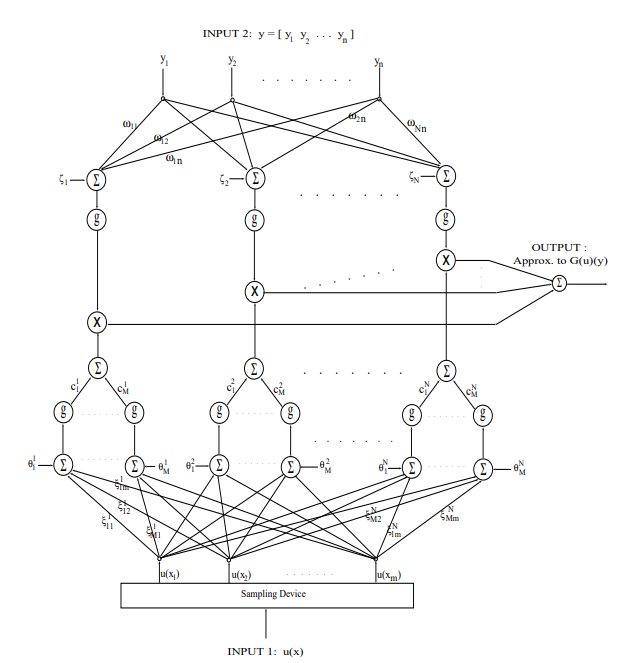
\includegraphics[width=1\textwidth]{img/img02.png}
    \caption{Arquitectura de red neuronal para la aproximación de operadores no lineales extraída de ~\cite{chen1995universal}.}
    \label{fig:img02}
\end{figure}
\endinput

